\chapter{Method\label{cha:chapter5}}

\section{Hypothesis \& Research Questions}
\label{sec:hypothesis}
To recall, previous research has not shown that it is possible to predict tap location on smartphone screen for data collected in a field environment. Due to this reason, data will be collected from both the field and the laboratory environment to investigate how classifiers, when trained with data from these environments, perform.
Initial assumptions are made that the environment has an effect on the classifier's prediction accuracy.
% In order to show this, a tap data set will be collected in the field as well as the laboratory environment. To show 
% As the feasibility of tap location inference has not been shown for data collected in the field environment, 
% To recall, previous research has shown that is it possible to predict location on a smartphone touch screen based on acceleromter and gyroscope recordings \cite{Tapprints, Accessory, Touchlogger}. However, since the data used for classification in these approaches was collected in a controlled environment, it has not been shown that the feasibility to predict tap locations also applies to a field environment. Therefore, data will be collected from both the field and the laboratory environments to investigate how classifiers, when fed with data from these environments, perform. Assumptions are made that the environment has an effect on the classifier's prediction accuracy.

\begin{center}
  \begin{mdframed}[backgroundcolor=gray!10] 
    \textbf{H.1}  The environment of recorded sensor data has an effect on the prediction accuracy.
  \end{mdframed}
\end{center}

In order to test the hypothesis stated above, a further assumption is made assuming that when a subject interacts with a smartphone screen, for instance, while walking or during a public transportation ride, the recorded sensory data will contain distortions which will, most likely, have a negative impact on the prediction accuracies. 

\begin{center}
  \begin{framed}
    \textbf{H1.1:} The prediction accuracy for a classifier trained with the data in the laboratory environment will score higher than one trained with data collected in the field.
  \end{framed}
\end{center}

Moreover, assumptions are made on the way the user interacts with the device. A user can either use the thumb to touch or the index finger while holding the device in the other hand. Assuming that the input modality also has an effect on the behavior of the estimator, data sets for both hands will be evaluated.

\begin{center}
  \begin{mdframed}[backgroundcolor=gray!10]
    \textbf{H2:} The input modality has an effect on the prediction accuracy.
  \end{mdframed}
\end{center}

It is plausible that tapping with the index finger, due to the force resistance of the supporting other hand, will cause less movement of the smartphone as typing with a thumb will. This is presumably to be reflected in the motion data.

\begin{center}
  \begin{framed}
    \textbf{H2.1:} The prediction accuracy for a classifier trained with index finger tap data will score higher than one trained with thumb tap data.
  \end{framed}
\end{center}

Finally, assumptions are made based on the body posture a user has while tapping. Overall, a difference in classification results is assumed between standing and sitting.
\begin{center}
  \begin{mdframed}[backgroundcolor=gray!10]
    \textbf{H3:} The body posture has an effect on the prediction accuracy.
  \end{mdframed}
\end{center}

To approve or reject this hypothesis, it is assumed that a user while sitting will move less compared to one who is standing which, as a result, will lead to a better predictability of the tap location.

\begin{center}
  \begin{framed}
    \textbf{H3.1:} The prediction accuracy for a classifier trained with taps where a user sat will score higher than one trained with taps where a user stood.
  \end{framed}
\end{center}

As a more severe scenario arises if an attacker could scale out the attack to predict tap locations of unseen users, a cross user experiment will be performed as a further step. For this purpose, the question is posed if it is possible to infer tap location of unseen users in the field with a classifier trained on laboratory data from different set of users.

\section{Experimental Approach}

\begin{figure}[h!]
  \centering
  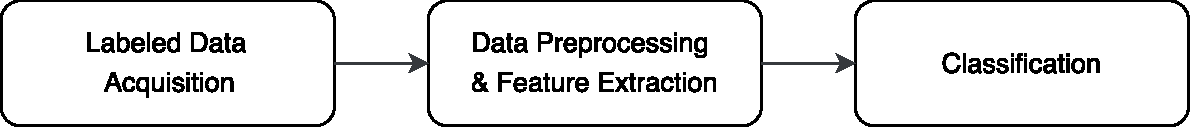
\includegraphics[width=1\textwidth]{approach2.pdf}
  \caption{This figure shows the overall approach to the experiment.} \label{fig:appraoch}
\end{figure}

The overall experiment consists of a three step process. In the first step, labeled data is acquired from subjects in the field and in the laboratory. For this purpose, the TapSensing application presented in the last chapter is used. The data acquisition part is a necessary step to collect sensor data with the corresponding ground truth of the tap locations for the supervised learning task. 

After the data is successfully acquired, the continuos sensor recordings are pre-processed to obtain the portion of recording which represents each individual tap. To extract certain characteristics of the sensor signature, feature are extracted in a further step. These features are then used to train a classifier.

In order to compare individual estimators, as for instance for the comparison between laboratory and field, a classifier will be evaluated using a k-fold cross-validation. The individual accuracy scores of the cross-validation are then compared by means of a Wilcoxon signed-rank test.

\section{Labeled Data Acquisition}

\subsection{Participants}
A total of 27 participants were invited to participate in the study. There were no restrictions concerning the demographics of individual subjects. However, each subjects had to be in  possession of one of the permitted iOS devices.

\subsection{Devices}
The devices have been restricted to the Apple iPhone 6, 6s and 7 based on their mutual screen size. Furthermore, as the screen size has a large effect on the sensor signature created by a tap, the screen size is an important factor to enable the comparison of classification results among devices.

\subsection{Environments \& Conditions}
As the study aims at collecting sensor reading both in the field as well as in a laboratory environment, the data acquisition is done in two distinct settings:

\begin{enumerate}
  \item \textbf{Laboratory Evironment}: Participants were invited to a laboratory room which had a standard office ergonomics setup. Participants have been asked to either sit at the desk or stand in the room while tapping.
  \item \textbf{Field Environment}: Participants were asked to generate taps using their smartphone at any place they are currently located. For example, this could be at home, at work or during leisure activity.
\end{enumerate}

Besides the environment of the recorded sensor data, the collected data varies in the input modality and body posture. Participants are either allowed to use the index finger (while holding the device in the other hand) or the thumb to generate taps. Sitting and standing are allowed as body postures as these two represent the natural interactions with the smartphone.

Regarding the distribution of the input modalities and body postures, in the laboratory part of the data acquisition, the input modality and body posture will be instructed for an equal distribution of both variables. In the field acquisition, however, the body posture and input modality can be decided by the participant in order to gain a more natural distribution of both factors.

\subsection{Survey}
In a short survey participants are asked about their basic demographics. This includes the age, gender, current occupation and if they are left or right-handed. In a further step, questions are asked regarding their personal smartphone usage. It is asked which device model they own, which input modalities they generally use and which input modality they use most often. Tapping with the index finger, tapping with the thumb or typing with both thumbs are considered as answer possibilities for the question concerning the input modality.

\subsection{Acquisition Procedure}
In order for participants to generate tap data, the subjects were invited to come to the laboratory for the first part of the experiment. To avoid information asymmetry, each participant read an experiment instruction\footnote{The instruction sheet is to be found in the appendix.}. Subjects should then confirm whether they have understood the previously read information. Additional questions regarding the instructions were answered. In the next step, subjects were asked to fill out an online questionnaire regarding their persona and personal smartphone usage.

% TODO: instruction in appendix
To begin with the data acquisition, participants were asked to download the application from the Apple App Store and to login using provided credentials.

\begin{figure}[h!]
  \centering
  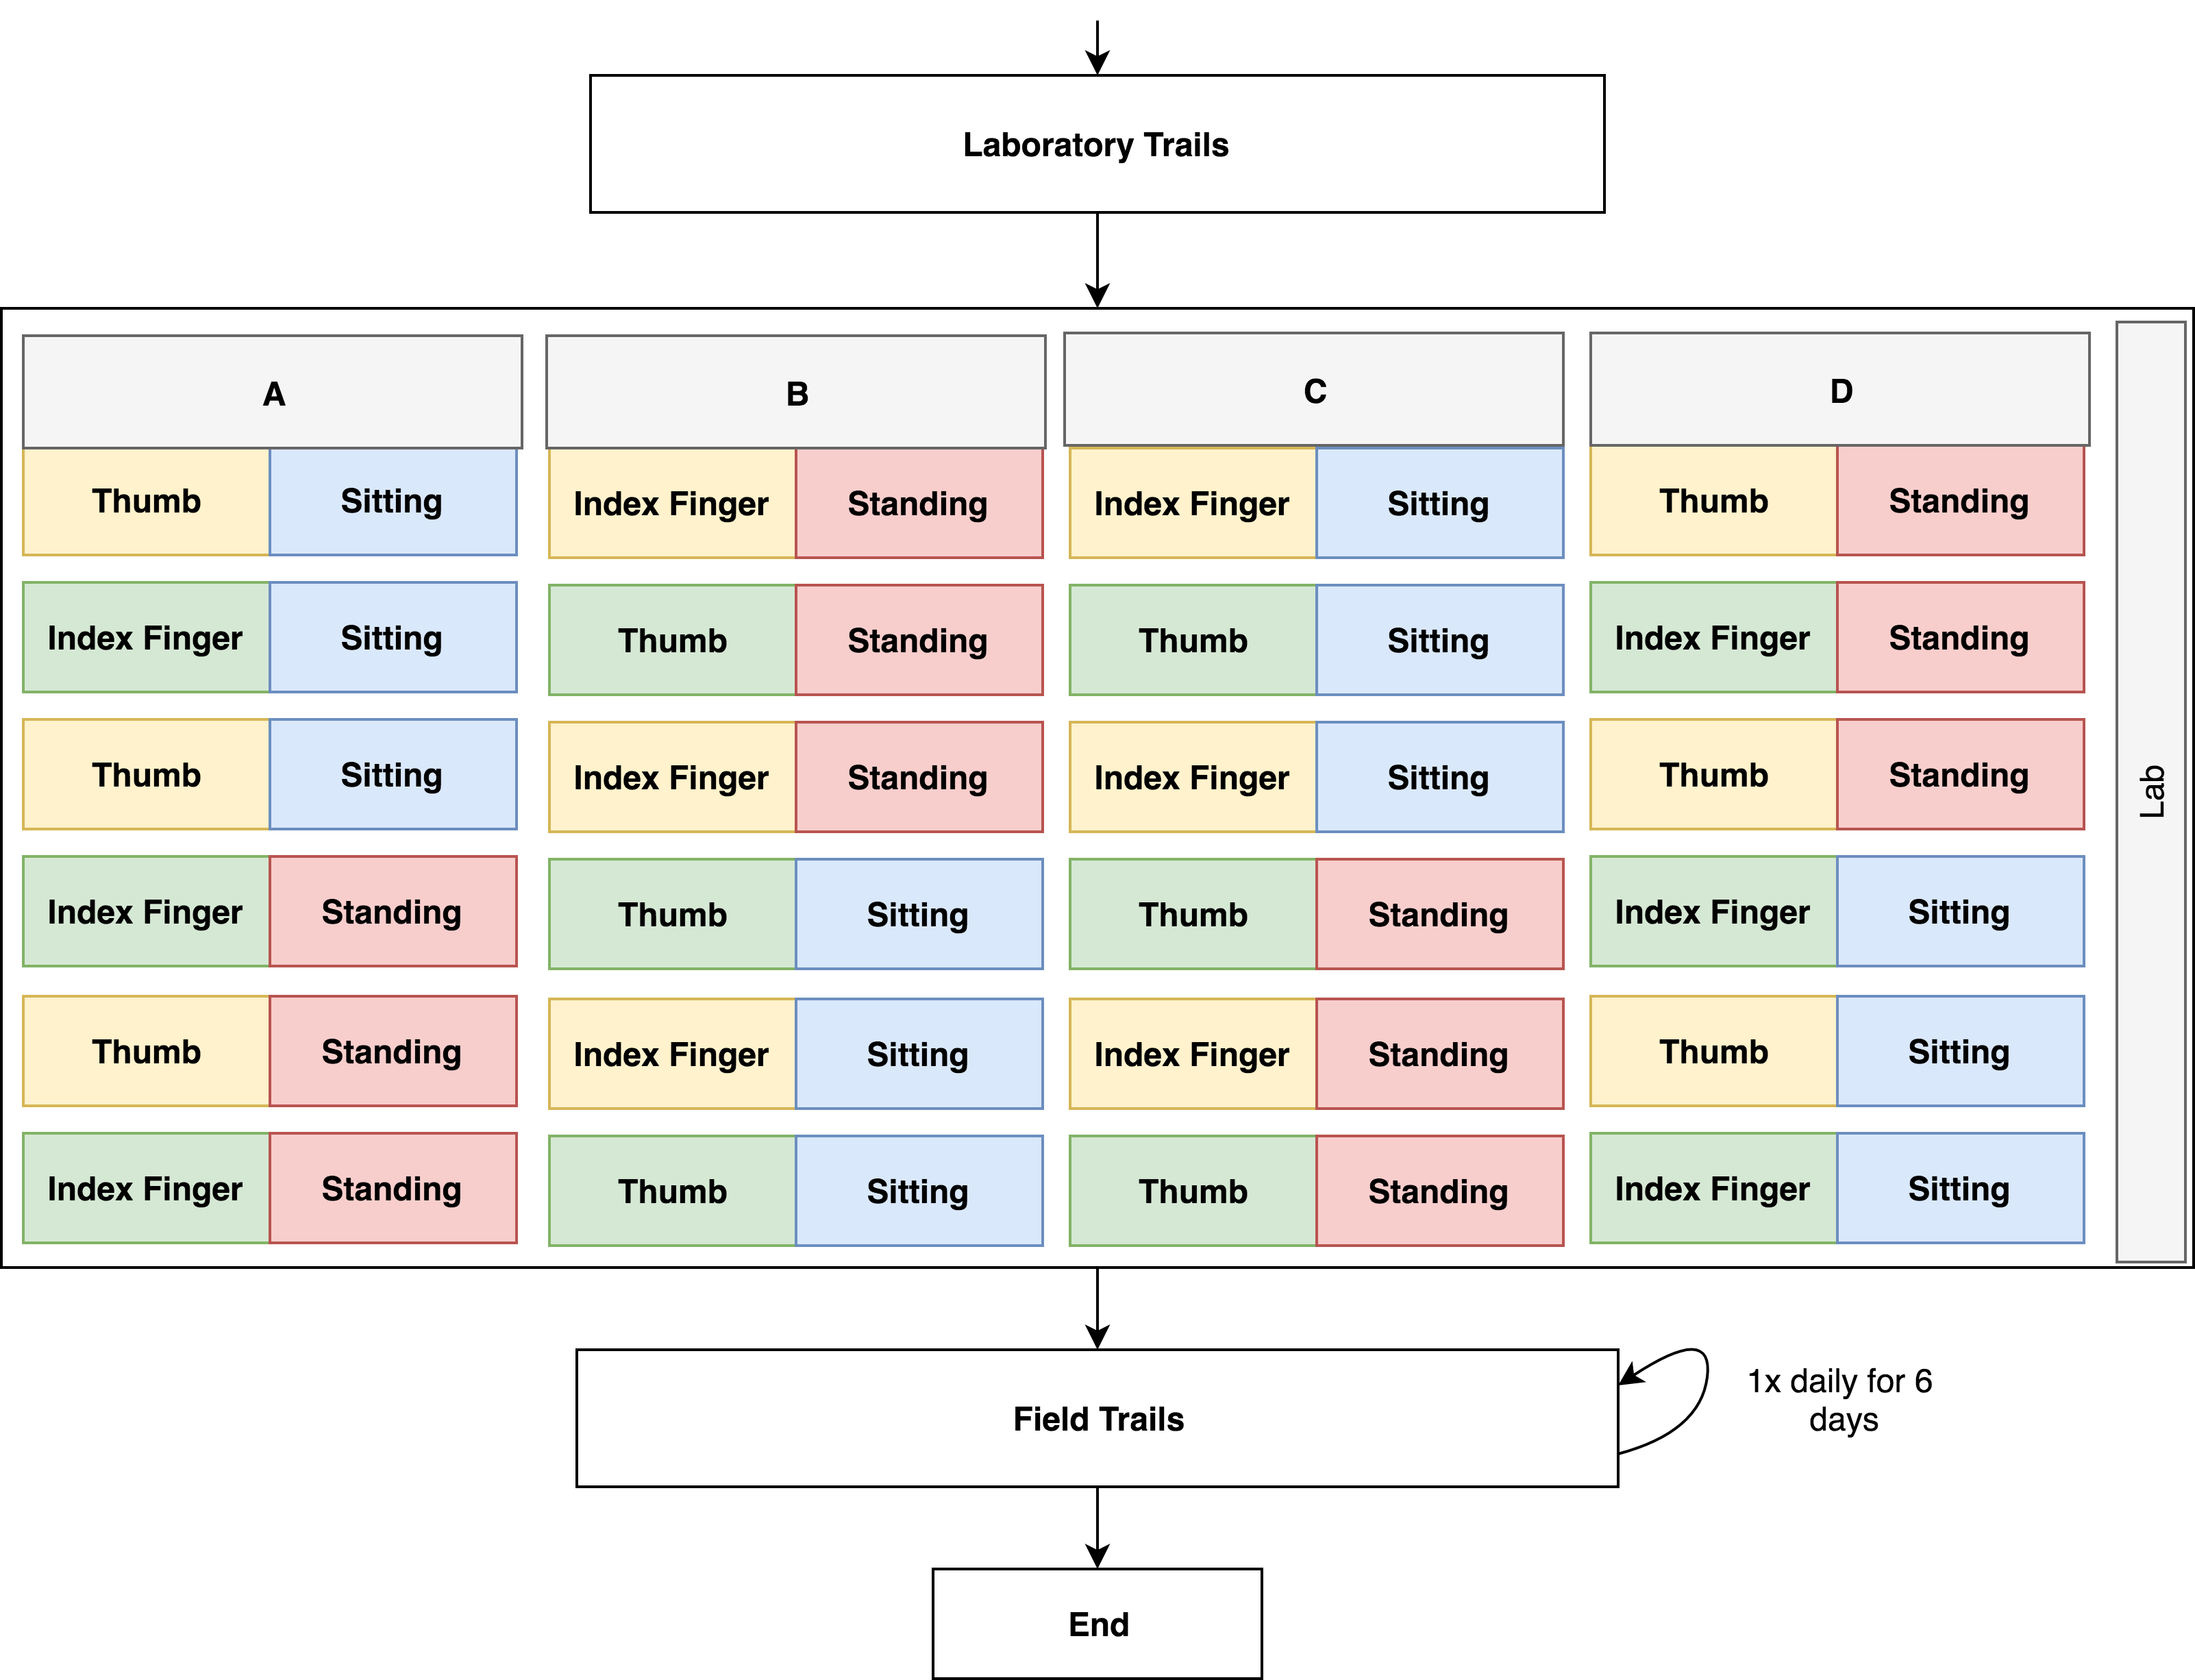
\includegraphics[width=1\textwidth]{study_design.png}
  \caption{This figure shows the procedure every subject has to perform in the study.} \label{fig:study_design}
\end{figure}

Subsequently, subjects were asked to perform 6 consecutive trials in the TapSensing application, whereas one trail includes tapping each grid four times in randomized order. Recall, the grid sizes defined consist of 4, 12 and 20 distinguishable buttons. For an equal distribution of the body posture and the input modality while tapping, each trial is dependent on one of four configurations onto which each subject is assigned. These configurations are to be seen in Figure \ref{fig:study_design} and have the advantage to minimize any learning effect the user has with the application. It is important to note that each subject is not allowed to alter the body posture or input modality during a trial. After all trials are performed, subjects were asked to continue with the field study.

During the field study, subjects performed one trial daily on 6 separate days. On each day push notifications were sent as a reminder to participate. Subjects were free to decide which input modality or body posture to use as the aim of the field study is to collect data that represents regular smartphone usage.

\section{Data Preprocessing \label{cha:chapter4}}
\subsection{Preprocessing}
Before features can be extracted from individual taps, the continuous sensor recording from each trial needs to be sliced to obtain the portion of the recordings which is relevant for the tap. The timestamp of the touchdown event is used to find an appropriate starting point. Here, 20ms are subtracted from the timestamp as due to the latency between the physical touchdown event and the recorded event. Based on the data collected in a pilot study, the average tap duration (being the duration between a touchdown and the corresponding touchup event) is between 70ms - 200ms. Taking this value into account, a window size of 150ms was chosen to enrich each slice with more information. Figure \ref{fig:touchdown} shows the sensor components of a gyroscope reading with a slicing window marked with a grey background. 

\begin{figure}[h!]
  \centering
  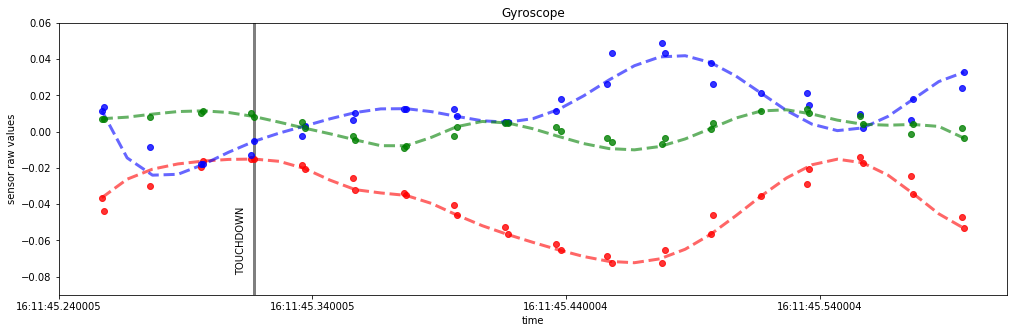
\includegraphics[width=1\textwidth]{gyroscope_touchdown.png}
  \caption{The figure shows a continuos gyroscope reading with the slicing window and corresponding timestamps. The timestamp of the touchdown event is used as an anchor point.} \label{fig:touchdown}
\end{figure}

Unfortunately, due to different CPU loads on the mobile devices, sensor values are not pushed from the operating system to the mobile application in a constant manner leading to an uneven distribution of the sensor recordings on the time scale. To balance out each tap to a fixed amount of values, a cubic spline interpolation is used. Figure \ref{fig:touchdown} shows the interpolated sensor components with dots representing the raw recordings. Furthermore, recordings that are below 75Hz are filtered out. After the slices are produced for each tap, features are extracted.

\subsection{Feature Extraction}
A feature is an individual measurable property or characteristic of a phenomenon being observed \cite{Duda:2000:PC:954544}. Therefore, choosing discriminant and independent features is a crucial step for the performance of the later classification. Fortunately, \citeauthor{Tapprints}'s preliminary work has shown a comprehensive list of possible sensor features of which the following features are partially adapted.

\begin{figure}[h!]
  \centering
  \begin{minipage}{.3\textwidth}
    \centering
    \begin{tikzpicture}
      \matrix [matrix of math nodes] (m)
      {
          g_{x_0} &g_{x_1} &g_{x_2} &g_{x_3} &g_{x_4} \\
          g_{y_0} &g_{y_1} &g_{y_2} &g_{y_3} &g_{y_4} \\            
          g_{z_0} &g_{z_1} &g_{z_2} &g_{z_3} &g_{z_4} \\
          \_ & \_ & \_ & \_ & \_ \\      
          a_{x_0} &a_{x_1} &a_{x_2} &a_{x_3} &a_{x_4} \\
          a_{y_0} &a_{y_1} &a_{y_2} &a_{y_3} &a_{y_4} \\            
          a_{z_0} &a_{z_1} &a_{z_2} &a_{z_3} &a_{z_4} \\
      };
      \draw[color=black!100, thick] (m-1-1.north west) -- (m-1-5.north east) -- (m-1-5.south east) -- (m-1-1.south west) -- (m-1-1.north west);
      \draw[color=black!100, thick] (m-2-1.north west) -- (m-2-5.north east) -- (m-2-5.south east) -- (m-2-1.south west) -- (m-2-1.north west);
      \draw[color=black!100, thick] (m-3-1.north west) -- (m-3-5.north east) -- (m-3-5.south east) -- (m-3-1.south west) -- (m-3-1.north west);
      \draw[color=black!100, thick] (m-5-1.north west) -- (m-5-5.north east) -- (m-5-5.south east) -- (m-5-1.south west) -- (m-5-1.north west);
      \draw[color=black!100, thick] (m-6-1.north west) -- (m-6-5.north east) -- (m-6-5.south east) -- (m-6-1.south west) -- (m-6-1.north west);
      \draw[color=black!100, thick] (m-7-1.north west) -- (m-7-5.north east) -- (m-7-5.south east) -- (m-7-1.south west) -- (m-7-1.north west);
      \node[align = center, below=2cm]{Column Features};
    \end{tikzpicture}
  \end{minipage}
  \begin{minipage}{.3\textwidth}
    \centering
    \begin{tikzpicture}
      \matrix [matrix of math nodes] (m)
      {
          g_{x_0} &g_{x_1} &g_{x_2} &g_{x_3} &g_{x_4} \\
          g_{y_0} &g_{y_1} &g_{y_2} &g_{y_3} &g_{y_4} \\            
          g_{z_0} &g_{z_1} &g_{z_2} &g_{z_3} &g_{z_4} \\
          \_ & \_ & \_ & \_ & \_ \\      
          a_{x_0} &a_{x_1} &a_{x_2} &a_{x_3} &a_{x_4} \\
          a_{y_0} &a_{y_1} &a_{y_2} &a_{y_3} &a_{y_4} \\            
          a_{z_0} &a_{z_1} &a_{z_2} &a_{z_3} &a_{z_4} \\
      };
      \draw[color=black!100, thick] (m-1-1.north west) -- (m-1-5.north east) -- (m-3-5.south east) -- (m-3-1.south west) -- (m-1-1.north west);
      \draw[color=black!100, thick] (m-5-1.north west) -- (m-5-5.north east) -- (m-7-5.south east) -- (m-7-1.south west) -- (m-5-1.north west);      
      \node[align = center, below=2cm]{Sensor Features};     
      % \draw[color=black,8oublies-](m-1-2.north) -- +(0,0.3);
    \end{tikzpicture}
  \end{minipage}
  \begin{minipage}{.3\textwidth}
    \centering
    \begin{tikzpicture}
      \matrix [matrix of math nodes] (m)
      {
          g_{x_0} &g_{x_1} &g_{x_2} &g_{x_3} &g_{x_4} \\
          g_{y_0} &g_{y_1} &g_{y_2} &g_{y_3} &g_{y_4} \\            
          g_{z_0} &g_{z_1} &g_{z_2} &g_{z_3} &g_{z_4} \\
          \_ & \_ & \_ & \_ & \_ \\      
          a_{x_0} &a_{x_1} &a_{x_2} &a_{x_3} &a_{x_4} \\
          a_{y_0} &a_{y_1} &a_{y_2} &a_{y_3} &a_{y_4} \\            
          a_{z_0} &a_{z_1} &a_{z_2} &a_{z_3} &a_{z_4} \\
      };
      \draw[color=black!100, thick] (m-1-1.north west) -- (m-1-5.north east) -- (m-7-5.south east) -- (m-7-1.south west) -- (m-1-1.north west);
      % \draw[color=red,double,implies-](m-1-2.north) -- +(0,0.3);
      \node[align = center, below=2cm]{Matrix Feature};
    \end{tikzpicture}
  \end{minipage}
  \caption{The figure shows how different features are extracted from the overall sensor matrices: Column features, sensor features and matrix features.}\label{fig:featureextraction}
\end{figure}  

The features extracted are differentiated based on the set of axis where aggregational functions are applied. These can be categorized as column features, sensor features and matrix features, as illustrated in figure \ref{fig:featureextraction}. Column features refer to features that are a product of a function being applied to each \textit{x}, \textit{y} and \textit{z} sensor axis separately. Sensor features are defined as features where sensor axis are combined. An example for a sensor feature is the Pearson correlation which is calculated for each sensor component pair \textit{xy}, \textit{xz} and \textit{yz}. With sensor features, relations between the components are captured. Lastly, matrix features are a product of a function being applied to both gyroscope and accelerometer time series.

Since taps on different locations of the screen generate different sensor signatures we design features that are able to capture the properties of the sensor readings generated by a tap. For this purpose, a total of 230 features have been extracted for each individual tap. The table \ref{table:features} below shows the complete list of features ordered by feature type. Features have been extracted from both the time domain and the frequency domain. In addition, to standardize the range of the features extracted, a Min-Max scaling is applied to each feature.
\newpage

\begin{center}
  % Feature Description
  \begin{longtable}{ | c | c | c | c | }
  \hline
  Name & Description & Feature Type & Amount \\
  \hline
  \endhead % all the lines above this will be repeated on every page
  \hline  
  \endfoot
  
    \texttt{peak} & Amount of peaks in the time series & column  & 6 \\
    \texttt{zero\_crossing} & Amount of zero crossings in the signal & column  & 6 \\ 
    \texttt{energy} & Energy of the signal & column  & 6 \\ 
    \texttt{entropy} & Entropy measure of the the signal & column  & 6 \\
    \texttt{mad} & Median absolute deviation of the signal & column  & 6 \\
    \texttt{ir} & Interquartile Range & column  & 6 \\
    \texttt{rms} & Root mean square of the signal & column  & 6 \\
    \texttt{mean} & Mean of the time series & column  & 6 \\
    \texttt{std} & Standard deviation of the time series & column  & 6 \\
    \texttt{min} & Minimum of the time series & column  & 6 \\
    \texttt{median} & Median of the time series & column  & 6 \\
    \texttt{max} & Maximal value of the time series & column  & 6 \\
    \texttt{var} & Variance of the time series & column  & 6 \\
    \texttt{skew} & Skewness of the time series & column  & 6 \\
    \texttt{kurtosis} & Kurtosis of the time series & column  & 6 \\
    \texttt{sem} & Standard error of the time series & column  & 6 \\
    \texttt{moment} & Moment in the time series & column & 6 \\
    \texttt{spline} & Spline interpolation of the signal & column  & 6*12 \\
    \texttt{fft} & Fast Fourier Transform & column  & 6*5 \\
  \hline
    \texttt{cos\_angle} & Cosine Angle of sensor component pairs & sensor & 6 \\
    \texttt{pears\_cor} & Pearson Correlation of component pairs & sensor & 6 \\
  \hline
    \texttt{fro\_norm} & Frobenius matrix norm & matrix & 1 \\
    \texttt{inf\_norm} & Infinity matrix norm & matrix & 1 \\
    \texttt{l2\_norm} & L2 matrix norm & matrix & 1 \\
    \hline
  \hline
  \end{longtable}
  \captionof{table}{Table of features extracted from every tap.}\label{table:features}
\end{center}

\section{Classification}
After the features are extracted for all the tap data acquired, learning algorithms are applied in order to measure the classification accuracy. In this experiment, a SVM with radial basis kernel is used as well as a feedforward artifical neural network.

\subsection{Evaluation}
To evaluate the classifiers trained in the classification part of the experiment, a K-fold cross-validation is used. In K-fold cross-validation, the training set is divided into K subsets of equal sizes. Sequentially, every subset is tested using the classifier trained on the remaining K-1 subsets. During this process, each pattern in the data set is predicted once. After K classifiers are trained, the mean of the accuracy scores is computed to determine how well the classifier performs.

\subsection{Grid Search}
In order to optimize the hyperparameters of each learning algorithm, a grid search is performed. A grid search is an exhausting search through a defined subset of the hyperparameter space for each algorithm. The subset of parameters are combined using the cartesian product in order to configure the classifier. To evaluate each classifier with a set of hyperparameters, a 5-fold cross validation is performed.

The parameters $C$ and $\gamma$ of the SVM RBF kernel are tested during the grid search using exponential growing sequences, a recommended method to find suitable parameters \cite{hsu2003practical}.
\begin{align}
  C &= \{ 2^{k} | k \in \{-3, -2, ..., 14, 15\} \}\\ 
  \gamma &= \{ 2^{k} | k \in \{-13, -12, ..., 2, 3\} \}
\end{align}
As for the SVM, hyperparameters are defined for the ANN. Presumably the most crucial parameter in an ANN is the amount of hidden layers defined. When a network is too large it tends to overfit the training data while a too small network can lead to high bias. Therefore, networks ranging from 2 to 12 hidden units are defined and evaluated during the grid search. To regularize the networks an $L_2$ penalty \cite{ng2004feature} is used. The following table \ref{table:anns} lists all configurations of the evaluated ANNs.

\begin{center}
  \begin{tabular}{ | l | l | l | l | l |}
  \hline
  Hidden units & L2 Penalty & Learning Rate & Activation & Optimizer \\ \hline
  12 & 0.001 & 0.01 & RELu & Adam \cite{DBLP:journals/corr/KingmaB14} \\
  10 & 0.003 & 0.01 & & \\
  8 & 0.0001 & 0.1 & & \\
  4 & 0.0003 & & & \\
  2 & & & & \\
  \hline
  \end{tabular}
  \captionof{table}{ANN configurations during grid search.}\label{table:anns}
\end{center}

After the grid search is computed, the best performing model with corresponding hyperparameters is used for analysis.
\subsection{Metrics}
As the amount of taps are equal for each subject and grid cell, the amount of training examples for each class is balanced. Therefore, the standard accuracy score for the classifier is used.
\begin{align}
  A &= \frac{TN + TP}{TN + FP + TP + FN} 
\end{align},
where TN is the number of true negative cases, FP is the number of false positive cases, FN is the number of false negative cases and TP is the number of true positive cases.
\raggedbottom
% parameter_candidates = [
%   {'hidden_layer_sizes': [
%       [1000, 500, 200, 100],
%       [400, 200, 50], 
%       [200, 100, 25], 
%       [100, 50, 10], 
%       [50, 10]],
%    'solver': ['adam'],
%    'alpha': [0.001, 0.003, 0.0001, 0.0003],
%    'activation': ['relu'],
%    'learning_rate_init': [0.001, 0.01, 0.1],
%    'max_iter': [10000],
% #          'verbose': [True]
%   }
% ]





% The traditional way of performing hyperparameter optimization has been grid search, or a parameter sweep, which is simply an exhaustive searching through a manually specified subset of the hyperparameter space of a learning algorithm. A grid search algorithm must be guided by some performance metric, typically measured by cross-validation on the training set[2] or evaluation on a held-out validation set.

